\documentclass{beamer}
\usetheme{metropolis}
\usepackage{appendixnumberbeamer}
\usepackage{booktabs}
\usepackage[scale=2]{ccicons}
\usepackage[utf8]{inputenc}
\usepackage{tabularx,colortbl} % Advanced table configurations
\usepackage{fontspec}
\usepackage{xcolor}
\usepackage{subcaption}

\newcommand{\gray}{\rowcolor[gray]{.90}} % Custom highlighting for the work experience and education sections

\definecolor{bg_metro}{RGB}{250,250,250}
\definecolor{bg_frametitle}{RGB}{232,232,232}
\definecolor{txt_metro}{RGB}{39,55,58}
\setbeamercolor{frametitle}{ fg=txt_metro , bg=bg_frametitle }

\metroset{progressbar=frametitle}

\makeatletter
\def\blfootnote{\xdef\@thefnmark{}\@footnotetext}
\makeatother

\newcolumntype{b}{X}
\newcolumntype{s}{>{\hsize=.3\hsize}X}
\newcolumntype{t}{>{\hsize=.15\hsize}X}

\newcounter{saveenumi}
\newcommand{\seti}{\setcounter{saveenumi}{\value{enumi}}}
\newcommand{\conti}{\setcounter{enumi}{\value{saveenumi}}}

\title{Simple Neural Networks for Image Classification}
\author{Giovanni Ballarin and Stefanie Bertele}
\institute{Presentation}
\date{2018}

\AtBeginSection[]{
	\begin{frame}
		\frametitle{Table of Contents}
		\tableofcontents[currentsection]
	\end{frame}
}

\begin{document}

\frame{\titlepage}

\section{Introduction}

\subsection{Introduction}

\begin{frame}
	\frametitle{Introduction}
	We base this Project on the paper "\textit{Digit Recognition Using Single Layer Neural Network with Principal Component Analysis}" by Vineet Singh, and Sunil Pranit Lal (2015). \\
	\vspace{1em}
	Their approach is to use Principal Component Analysis to "compress" the number of features of the MNIST dataset, and then feed them into a neural network with 1 hidden layer for classification. We follow their approach in part, but we also expand on it.
\end{frame}

\subsection{Motivation}

\begin{frame}
	\frametitle{Motivation}
	Image classification tasks are the first class of visual recognition problems that one has to tackle in computer vision. While the set up in many cases is remarkably easy, lots of effort has been put into devising effective classification algorithms. \\
	\vspace{2em}
	Even a basic dataset like MNIST can be complex to classify if it is not approached with the "correct" tools. It is thus important to study what constitutes the \textit{minimal} set of techniques necessary to solve 
\end{frame}

\subsection{Datasets}

\begin{frame}
	\frametitle{Datasets}
	We consider the following datasets:
	\vspace{1em}
	\begin{itemize}
		\item MNIST
		\vspace{1em}
		\item notMNIST
		\vspace{1em}
		\item Fashion MNIST
	\end{itemize}
	\vspace{1em}
	Each consists of $28\times28$ pixels images that belong to 10 classes.
\end{frame}

\begin{frame}
	\frametitle{MNIST}
	\begin{figure}[hbt]
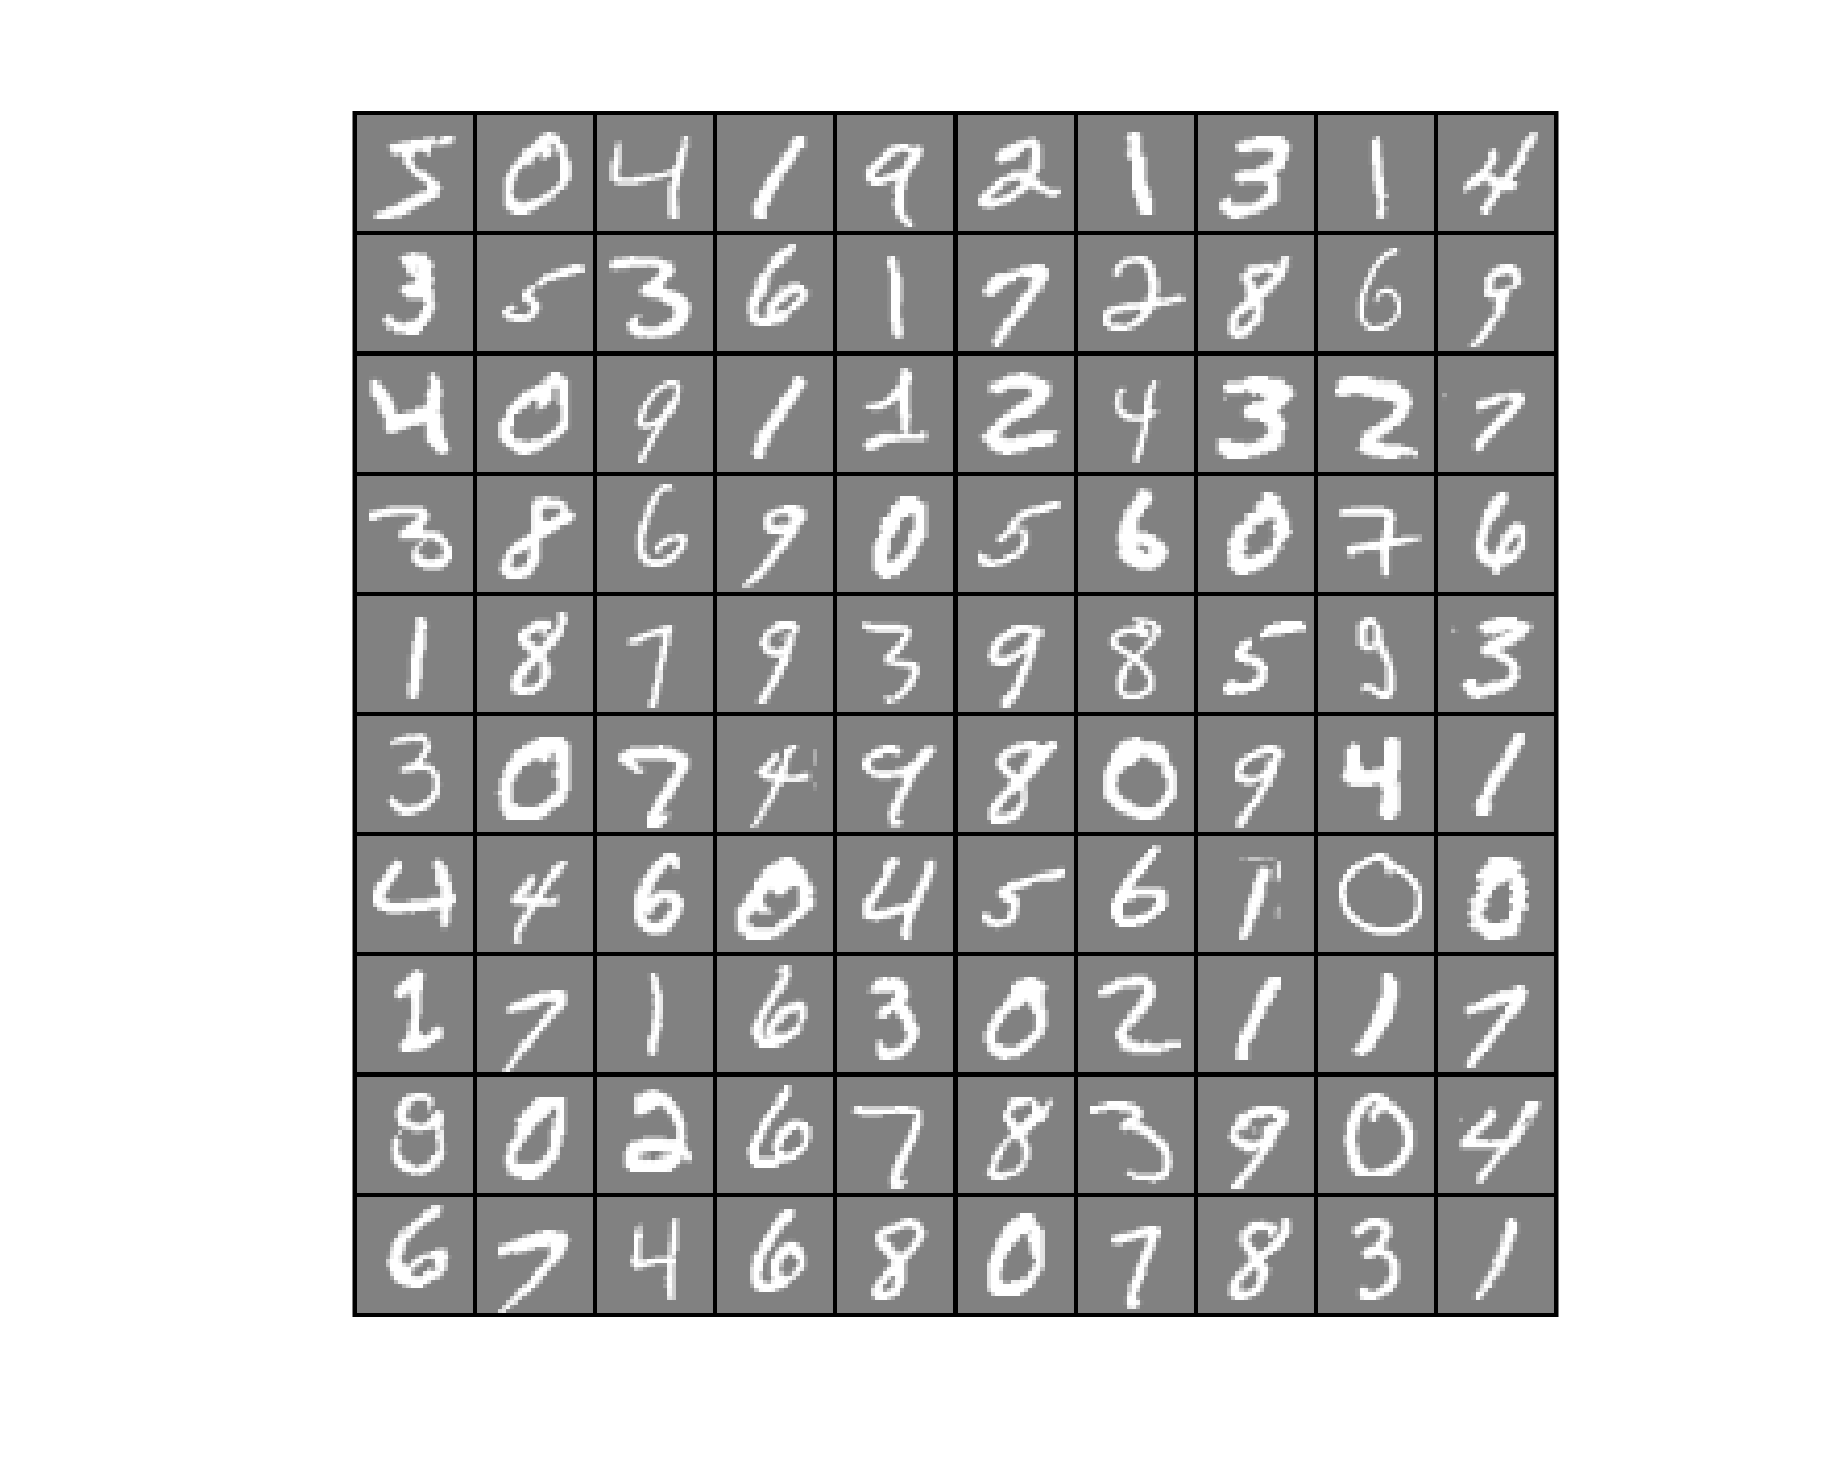
\includegraphics[width=1\textwidth,height=0.8\textheight,keepaspectratio]{mnist_example}
  	\caption{\footnotesize{Example images from the MNIST dataset.}}
	\end{figure}
\end{frame}

\begin{frame}
	\frametitle{notMNIST}
	\begin{figure}[hbt]
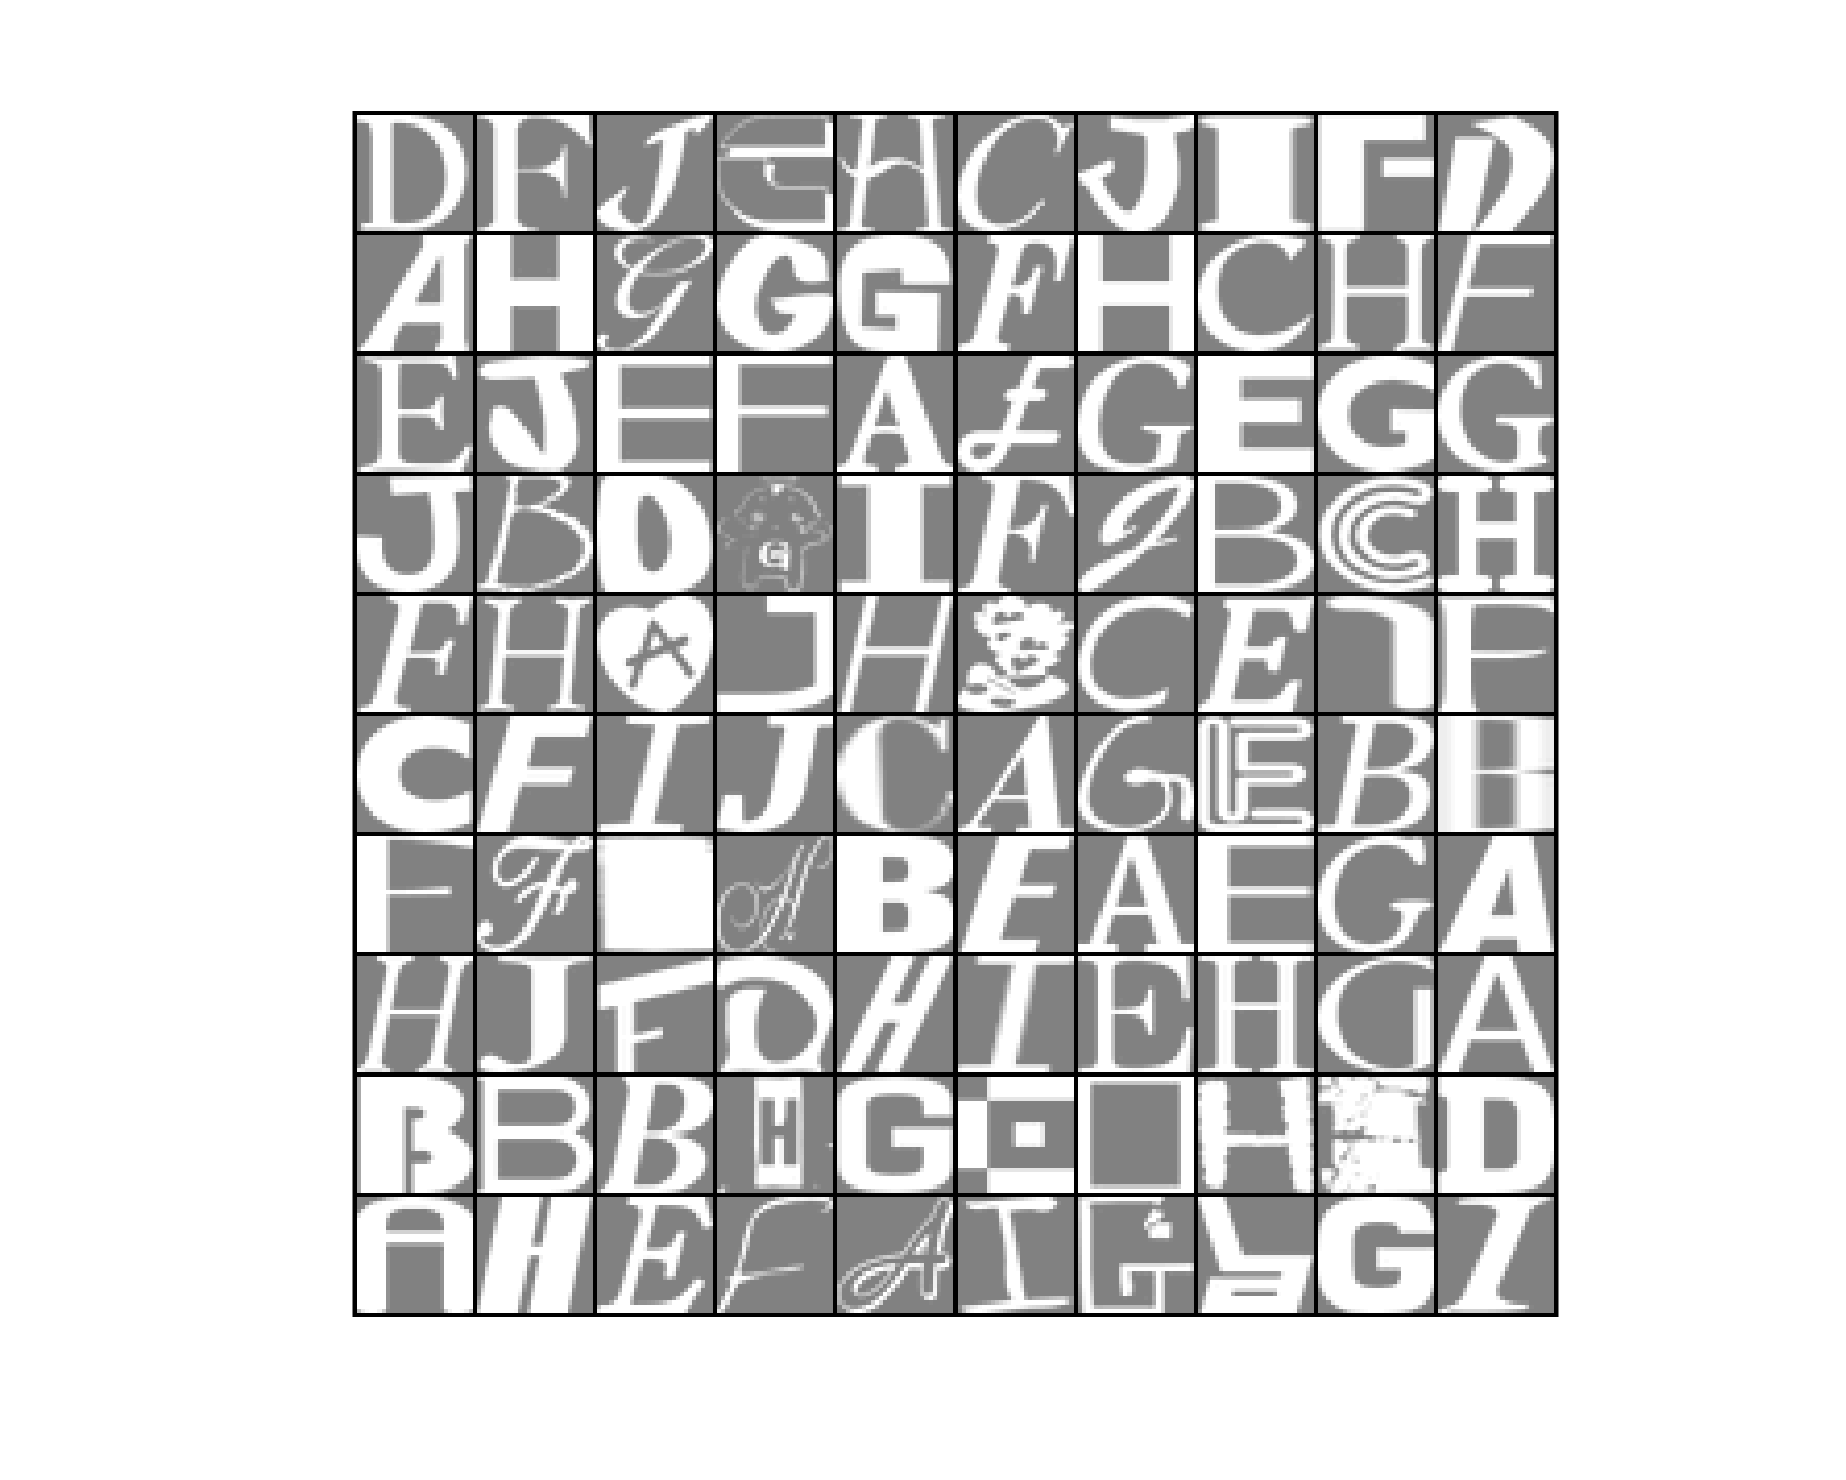
\includegraphics[width=1\textwidth,height=0.8\textheight,keepaspectratio]{notMnist_example}
  	\caption{\footnotesize{Example images from the notMNIST dataset.}}
	\end{figure}
\end{frame}

\begin{frame}
	\frametitle{Fashion MNIST}
	\begin{figure}[hbt]
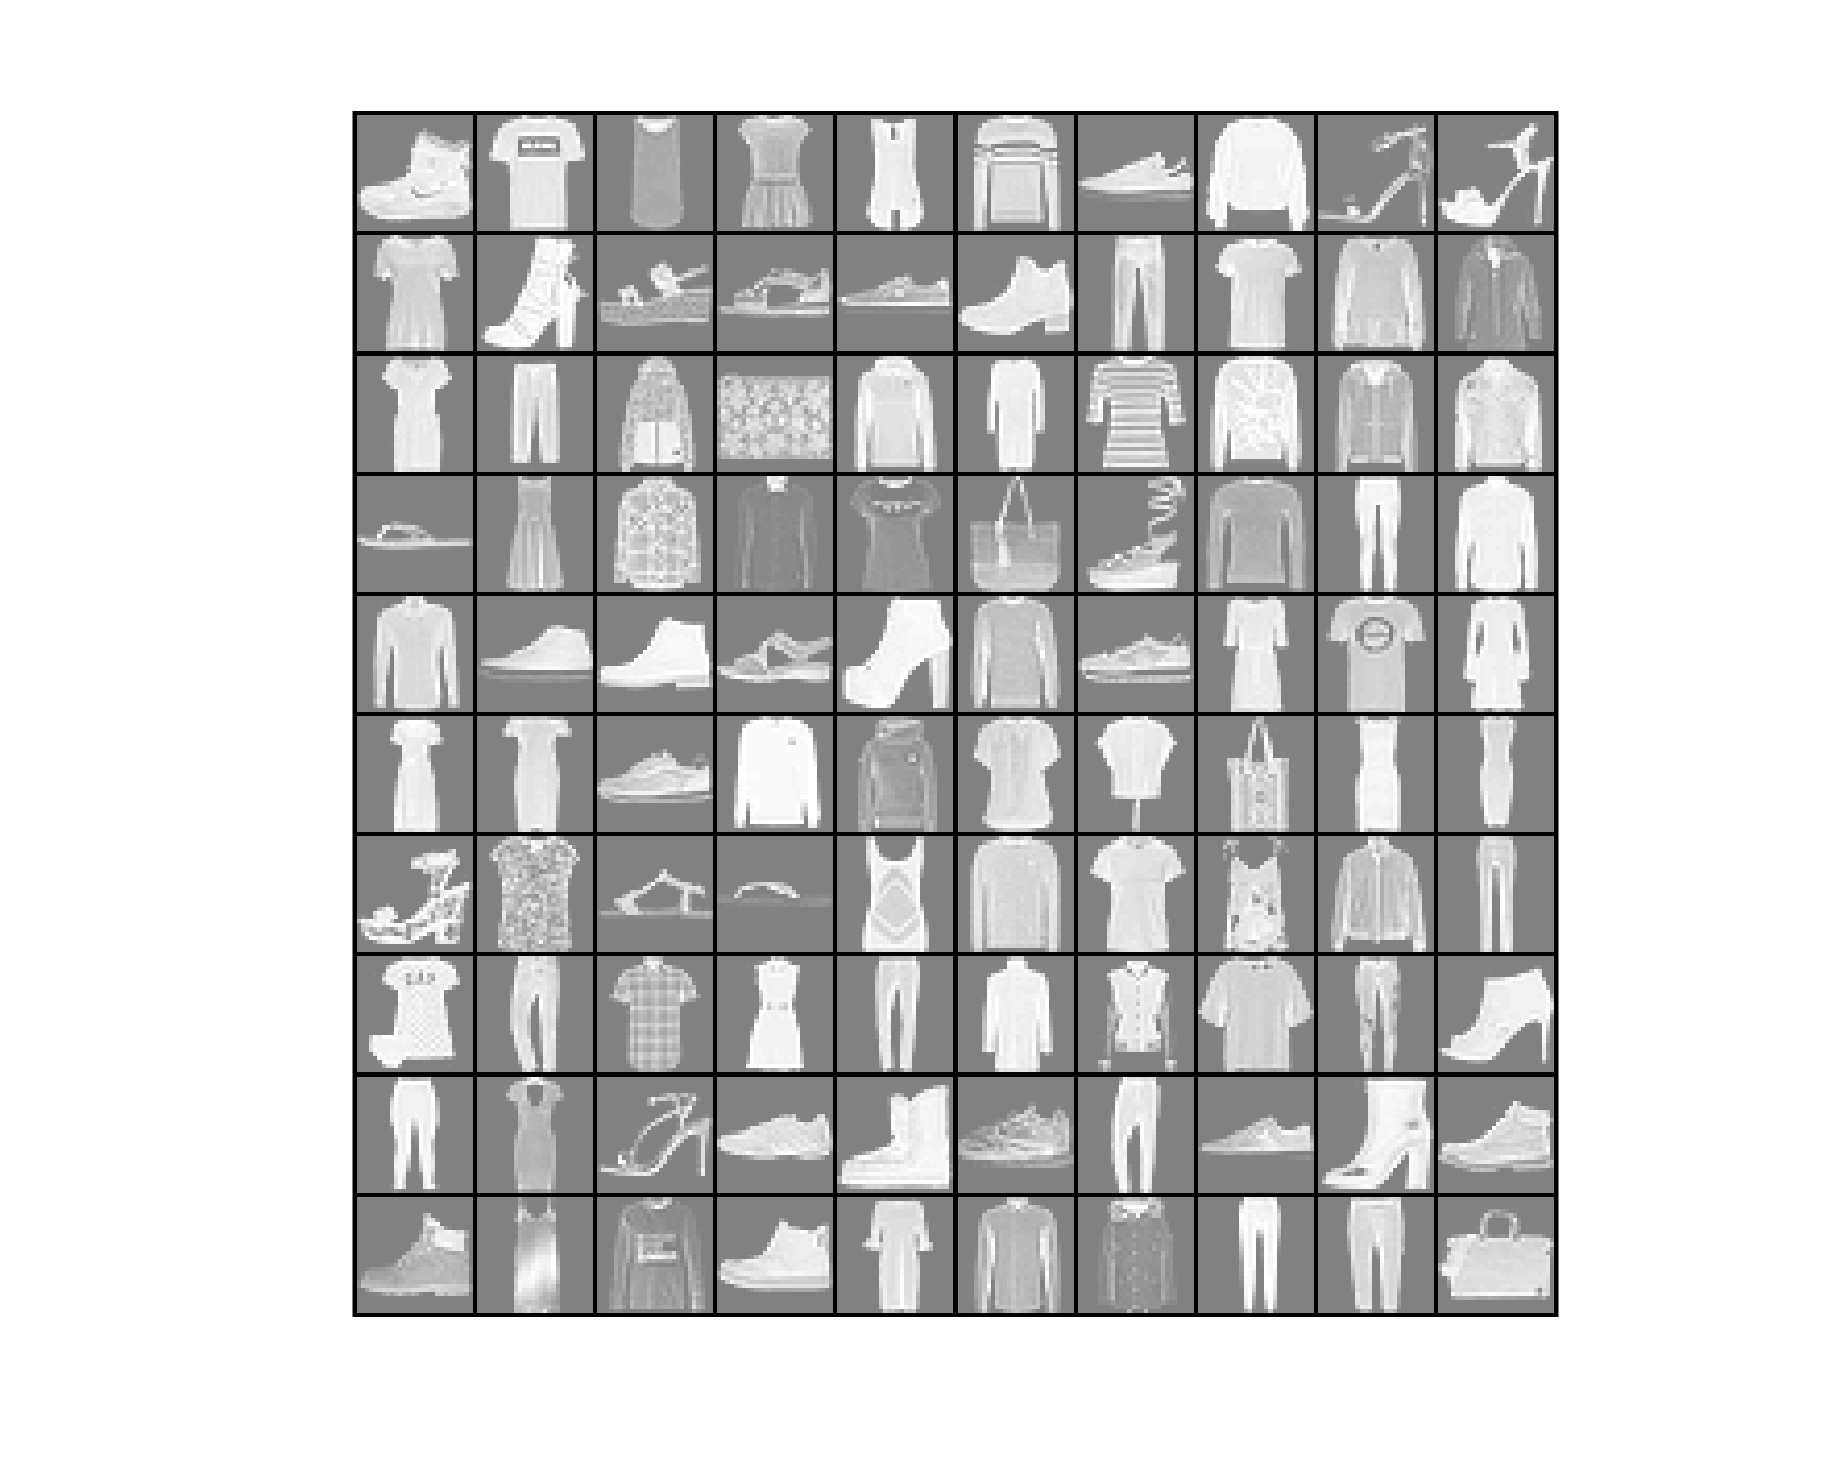
\includegraphics[width=1\textwidth,height=0.8\textheight,keepaspectratio]{fashion_example}
  	\caption{\footnotesize{Example images from the Fashion MNIST dataset.}}
	\end{figure}
\end{frame}

\section{Techniques}

\begin{frame}
	\frametitle{Approach}
	The following techniques:
	\begin{itemize}
		\item \textbf{PCA + 1D Neural Network} \\ 
			\textit{Idea}: Reduce the dimensionality of the $784\times1$ vector obtained from each image by projecting it into a smaller vector space, then classify it with a NN;
		\vspace{1em}
		\item \textbf{Convolutional Neural Networks} \\
			\textit{Idea}: Account for the spatial nature of the image by using a 2D Neural Network architecture;
	\end{itemize}
\end{frame}

\subsection{Principal Component Analysis}

\begin{frame}
	\frametitle{Principal Component Analysis - PCA}
	PCA is widely used as a projection technique to reduce the dimensionality of data. \\ The algorithm is straightforward:
	\begin{enumerate}
		\item Demean the data: $\overline{X} = X - m(X)$
		\item Compute the covariance matrix: \[ C = \frac{1}{N}\,\overline{X}\,\overline{X}^{\top}\]
		\item Find the eigenvectors (and eigenvalues) matrices, $V$ and $D$: \[ V^{\,-1}\,C\,V = D \]
		\item Order the eigenvectors by highest associated eigenvalue and project the data $X$ onto the first $K$ components: \[ Z = \overline{X}\,V(1:K) \]
	\end{enumerate}
\end{frame}

\begin{frame}
\frametitle{PCA - An Example}
	\begin{figure}[hbt]
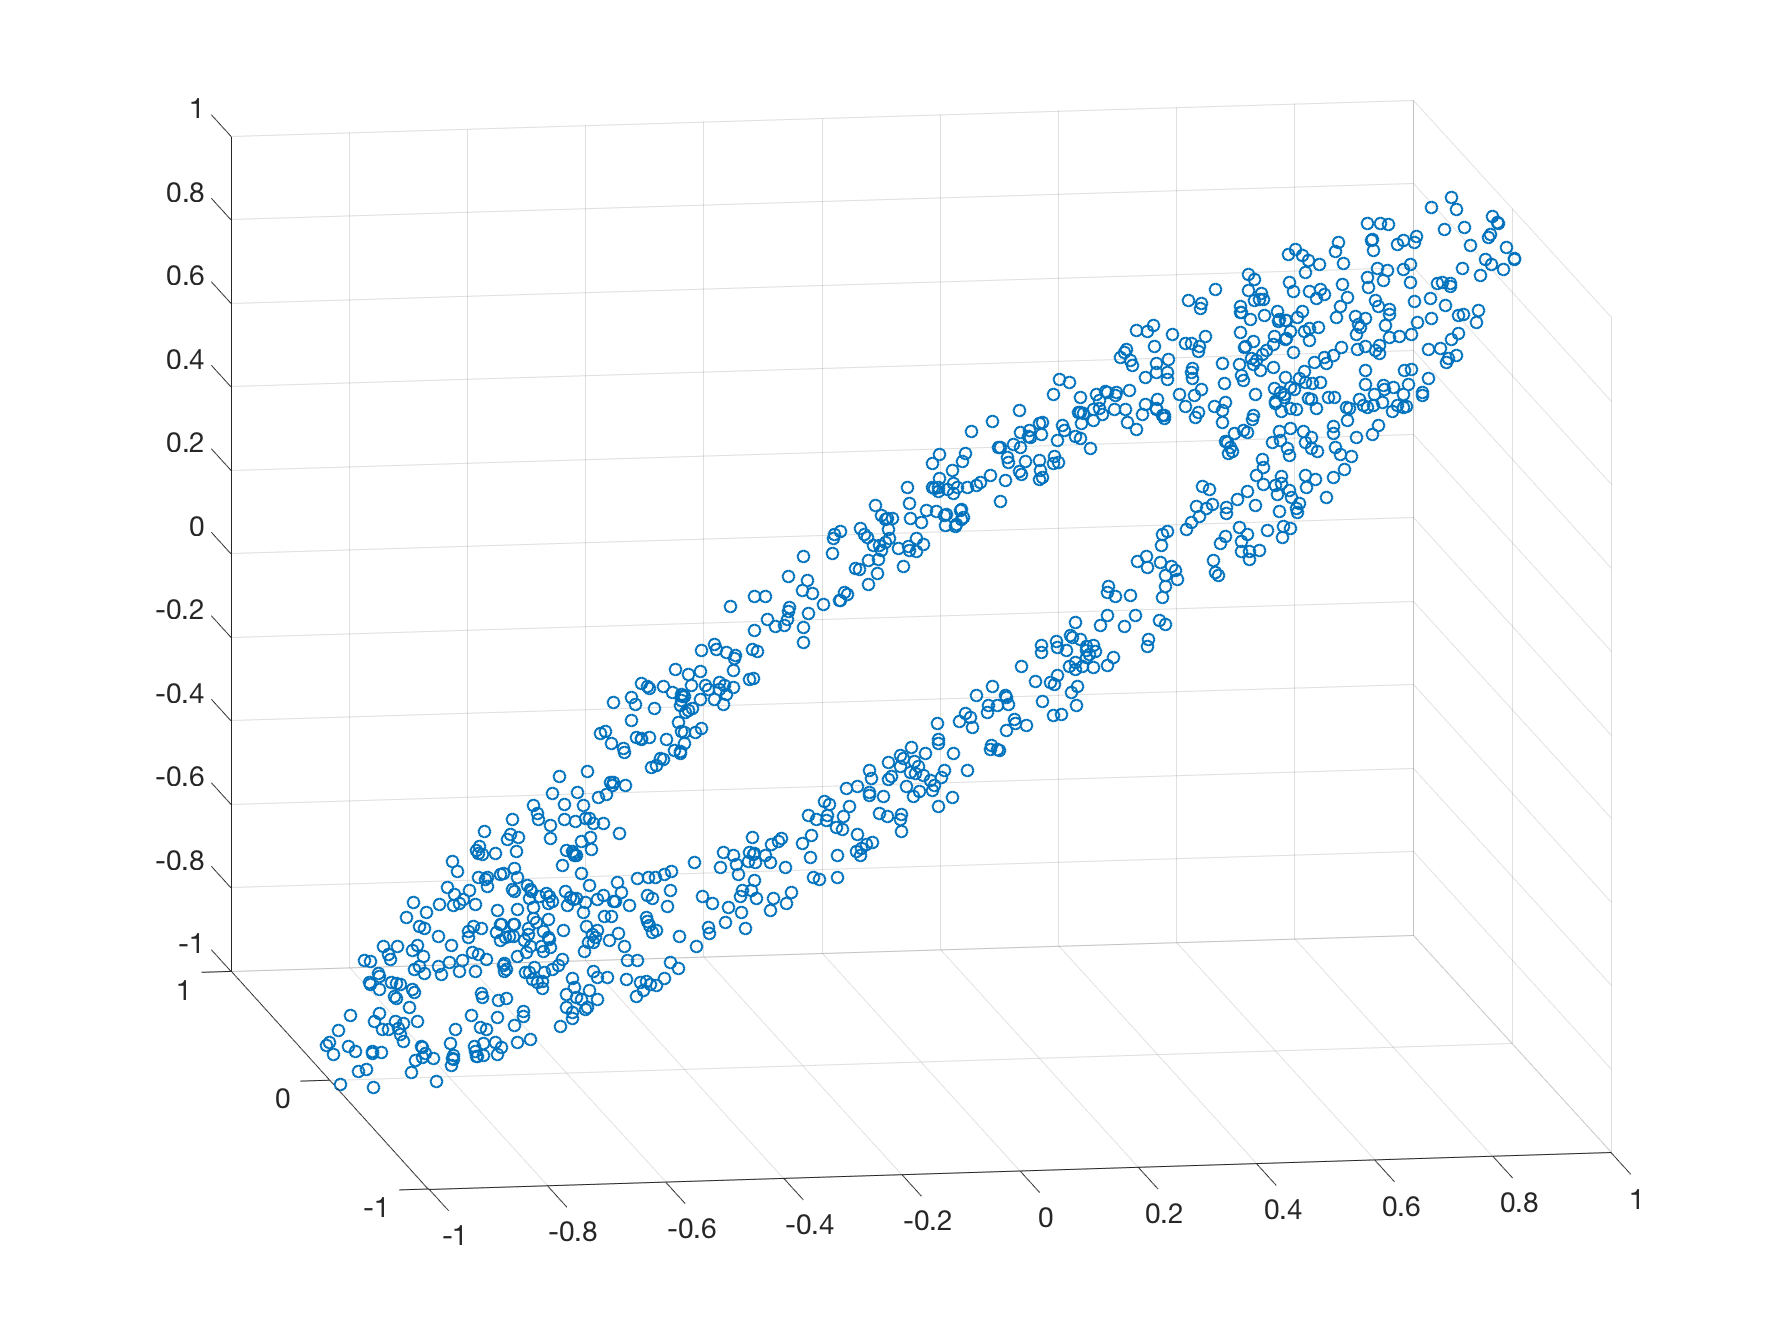
\includegraphics[width=1\textwidth,height=0.7\textheight,keepaspectratio]{ring_3d}
  	\caption{\footnotesize{A "3D Ring" point cloud before PCA.}}
	\end{figure}
\end{frame}

\begin{frame}
\frametitle{PCA - An Example}
	\begin{figure}[hbt]
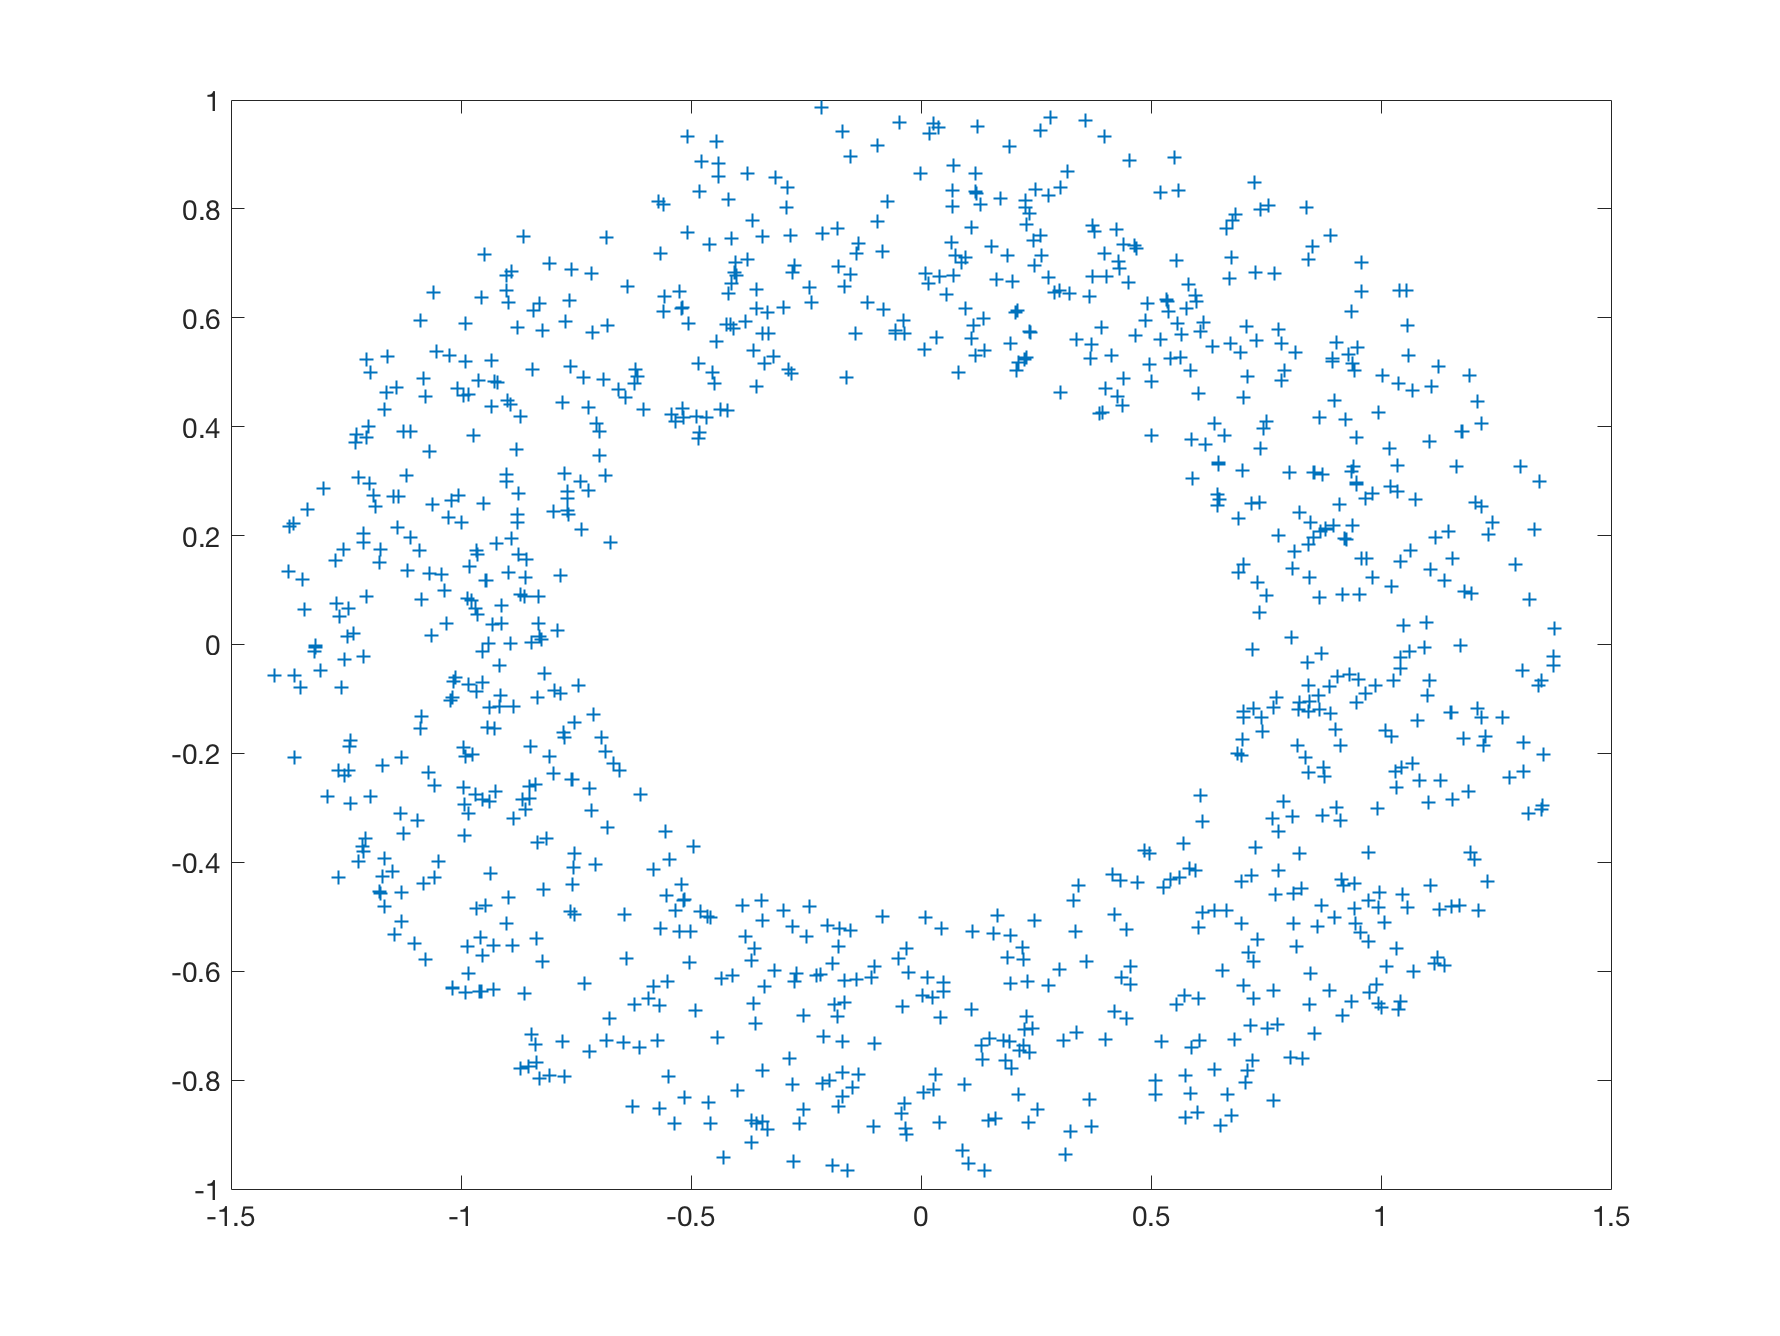
\includegraphics[width=1\textwidth,height=0.7\textheight,keepaspectratio]{ring_pca}
  	\caption{\footnotesize{PCA projects the "3D Ring" point cloud to 2D by removing the planar dimension.}}
	\end{figure}
\end{frame}


\begin{frame}
\frametitle{Architecture}
	\vspace{1em}
	PCA sizes \\
	\begin{itemize}
		\item 10
		\item 25
		\item 50
		\item 100
	\end{itemize}
	Fully connected NN architectures\\
	\begin{itemize}
		\item 10
		\item 25
		\item 100
		\item $25 \longmapsto 15$
		\item $25 \longmapsto 20 \longmapsto 15$
		\item $100 \longmapsto 50 \longmapsto 20$
	\end{itemize}
\end{frame}

\subsection{Convolutional Neural Networks}

\begin{frame}
	\frametitle{Convolutional Neural Networks - CNNs}
	CNNs are a variation of multilayer perceptrons that were designed to mimic the visual processing of living organisms. \\
	\vspace{1em}
	Each CNN layer has a number of \textbf{filters}: each filter is used to make a convolution with the image, producing a filter bank. The output of the convolutional layer is simply the collection of filter banks. \\
	\vspace{1em}
	CNNs have notable advantages compared to fully-connected NN:
	\begin{itemize}
		\item Filters are usually small in size (e.g. $5\times5$), thus they have considerably less parameters to train;
		\item CNNs preserve the spatial nature of 2D signals like images or video, thus allowing for more effective feature recognition.
	\end{itemize} 
\end{frame}


\begin{frame}
\frametitle{CNN - Architecture 1}
	\begin{figure}[hbt]
	\vspace{2em}
  	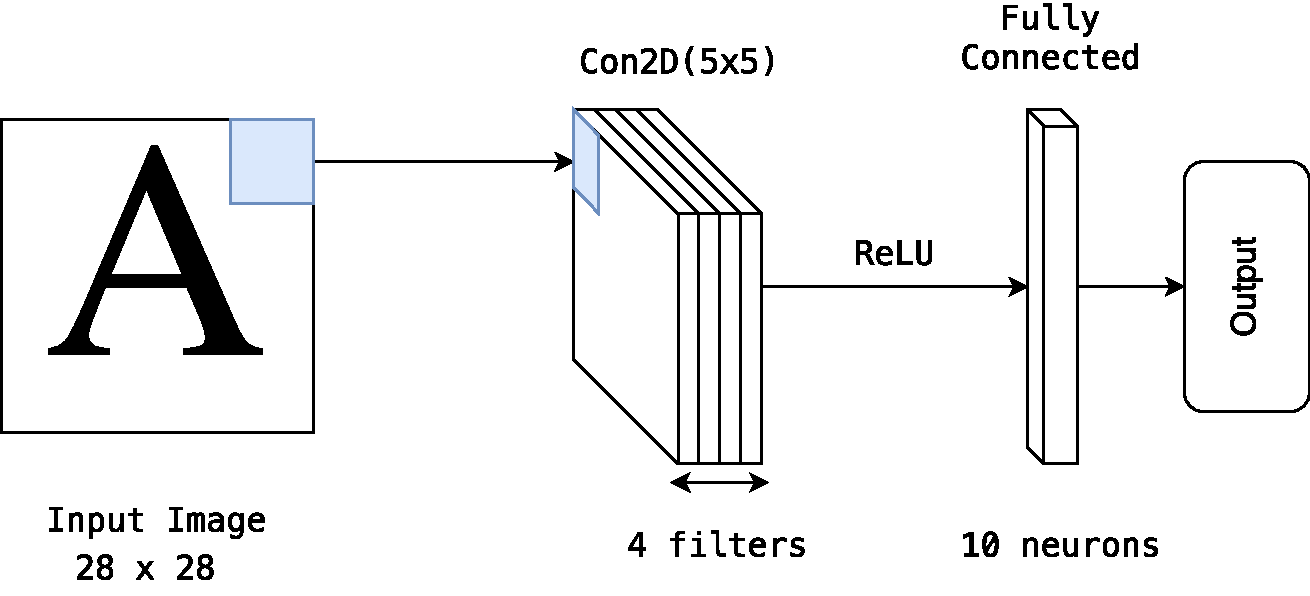
\includegraphics[width=1\textwidth,height=0.7\textheight,keepaspectratio]{diag_1}\\
    \vspace{2em}
  	%\caption{\footnotesize{CNN architecture 1}}
	\end{figure}
\end{frame}

\begin{frame}
\frametitle{CNN - Architecture 2}
	\begin{figure}[hbt]
	\vspace{2em}
  	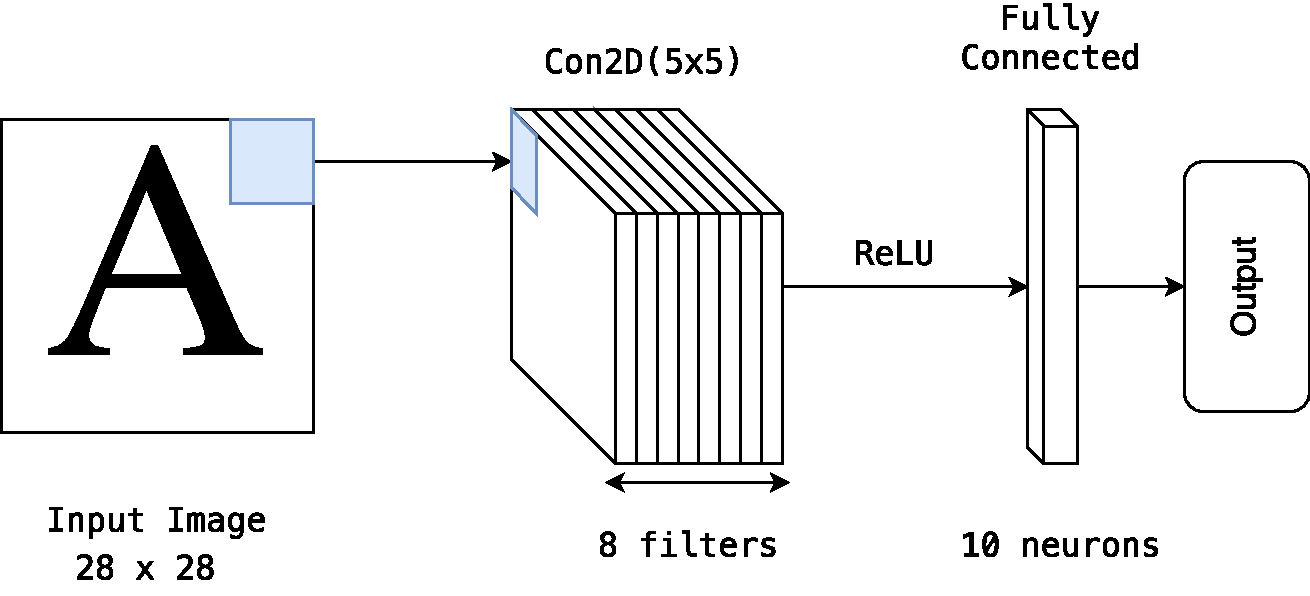
\includegraphics[width=1\textwidth,height=0.7\textheight,keepaspectratio]{diag_2}\\
    \vspace{2em}
  	%\caption{\footnotesize{CNN architecture 2}}
	\end{figure}
\end{frame}

\begin{frame}
\frametitle{CNN - Architecture 3}
	\begin{figure}[hbt]
	\vspace{2em}
  	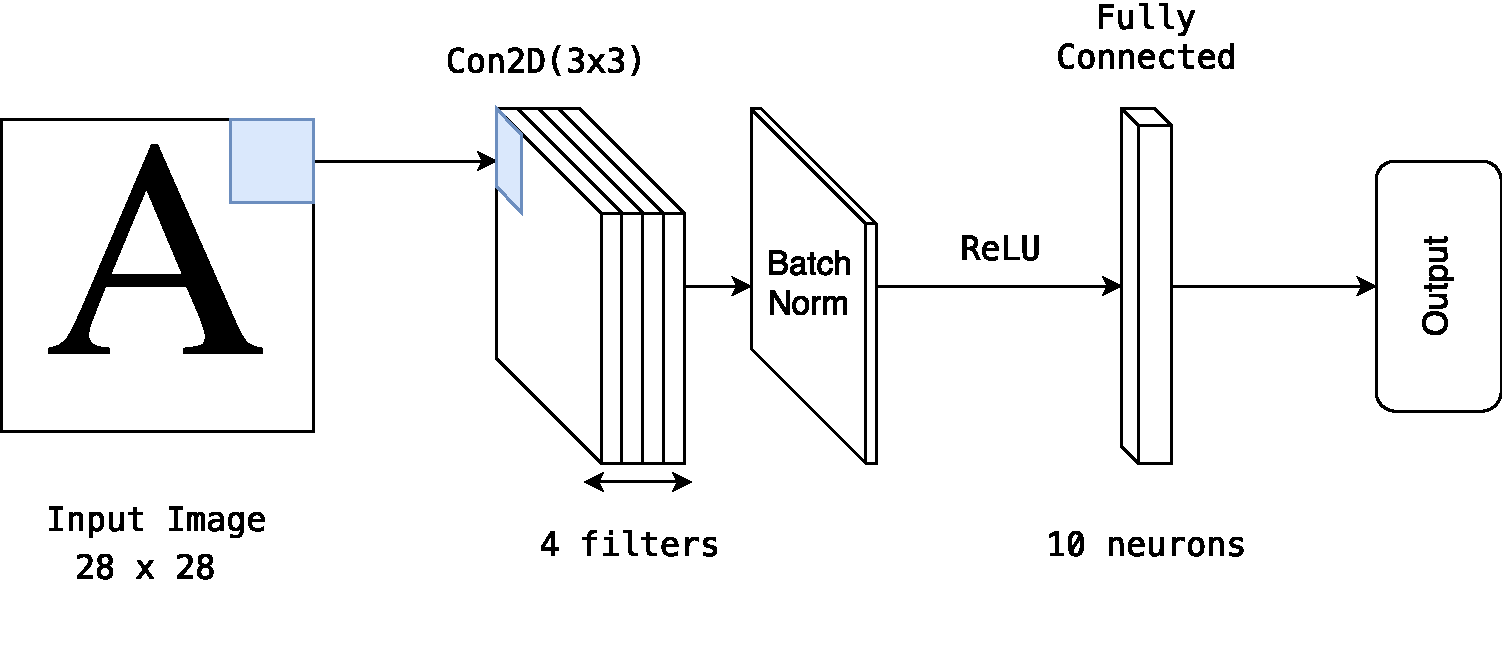
\includegraphics[width=1\textwidth,height=0.7\textheight,keepaspectratio]{diag_3}\\
    \vspace{2em}
  	%\caption{\footnotesize{CNN architecture 3}}
	\end{figure}
\end{frame}

\begin{frame}
\frametitle{CNN - Architecture 4}
	\begin{figure}[hbt]
	\vspace{2em}
  	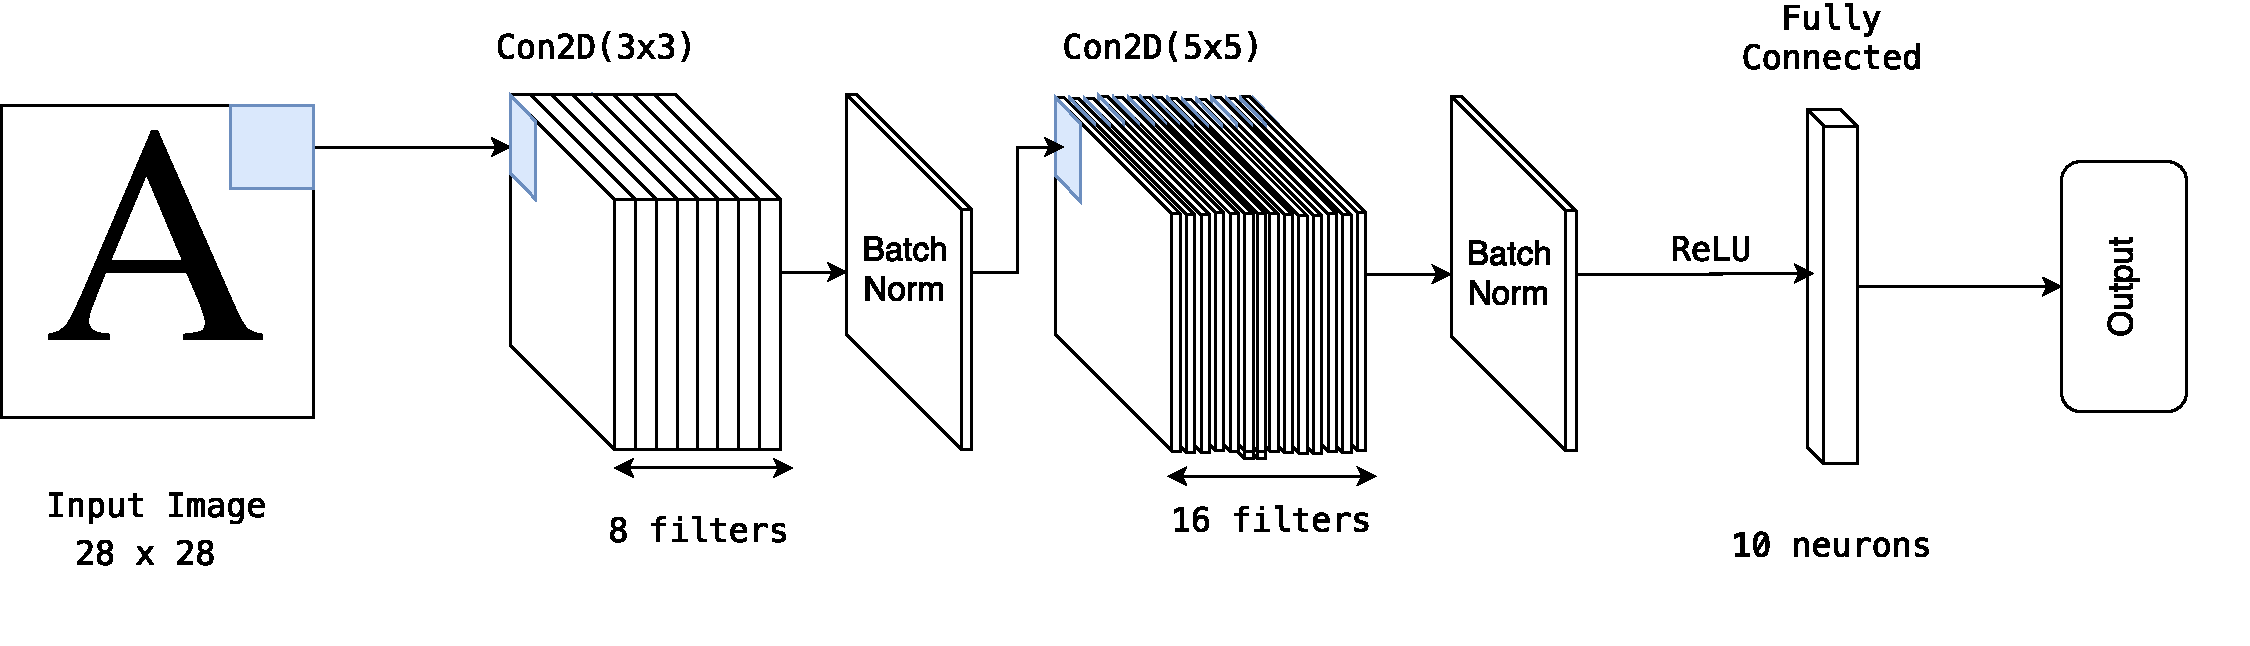
\includegraphics[width=1\textwidth,height=0.7\textheight,keepaspectratio]{diag_4}\\
    \vspace{2em}
  	%\caption{\footnotesize{CNN architecture 4}}
	\end{figure}
\end{frame}

\section{Results}

\subsection{PCA + 1D NN}

\begin{frame}[standout]
	\centering
	\textit{Results}\\
	\vspace{2em}
	\textbf{PCA + 1D NN}
\end{frame}

\begin{frame}
\frametitle{Results - PCA + 1D Neural Network - MNIST}
\begin{table}[hbt]
  \begin{tabular}{|cc|l|c|c|}
  	\hline
    \% Var & PCs & NN Architecture & Training Error & Test Error \\
    \hline
    \hline
    50 & 11 & 25 & 0.168   &  0.698 \\
    50 & 11 & 25-20-15 & 0.119  &   0.838  \\
    \hline
    75 & 33 & 25 & 0.088  &   0.729 \\
    75 & 33 & 100 &    0.037  &   0.817\\
    \hline
    85 & 58 & 10 & 0.084  &   0.705\\
    85 & 58 & 25-20-15 & 0.066  &   0.807\\
    \hline
    95 & 150 & 25 &  0.054   &  0.688\\
    95 & 150 & 100-50-20 & 0.049   &  0.852\\
    \hline
  \end{tabular}
  \vspace{1em}
  \caption{Best and worst results for different PCA sizes depending on explanatory power of the variance. Training size: 9000 images. Test size: 1000 images.}
\end{table}
\end{frame}

\begin{frame}
\frametitle{Results - PCA + 1D Neural Network - notMNIST}
\begin{table}[hbt]
  \begin{tabular}{|cc|l|c|c|}
  	\hline
    \% Var & PCs & NN Architecture & Training Error & Test Error \\
    \hline
    \hline
    50 & 5 & 100-50-20 & 0.207    & 0.612\\
    50& 5 & 25-20-15 & 0.235    & 0.639\\
    \hline
    75 & 19 &  100 & 0.089    & 0.555\\
    75 & 19& 25-20-15 & 0.104    & 0.642\\
    \hline
    85 & 40 & 25 & 0.101   &  0.559\\
    85 & 40 & 100-50-20 & 0.094     & 0.62\\
    \hline
    95 & 126 & 25-20-15 & 0.089   &  0.568\\
    95 & 126 & 25-15 & 0.081   &  0.587\\
    \hline
  \end{tabular}
    \vspace{1em}
  \caption{Best and worst results for different PCA sizes depending on explanatory power of the variance. Training size: 9000 images. Test size: 1000 images.}
\end{table}
\end{frame}

\begin{frame}
\frametitle{A Trick - 2D Fourier Transform}
	For the Fashion MNIST dataset, directly applying PCA and a fully-connected 1D neural network produces \textit{very bad results}. The final test error for all combinations is around \textbf{70\%}. \\
	\vspace{1em}
	A simple trick allows to reduce greatly the error: pre-treat the dataset with a 2D Fourier Transform on the images to move to the frequency domain. \\
	\vspace{1em}
	\textit{We loose the spatial information, but we reduce the test error by up to \textbf{30} percentage points!}
\end{frame}

\begin{frame}
\frametitle{A Trick - 2D Fourier Transform}
	\begin{figure}[hbt]
\begin{subfigure}{.5\textwidth}
  \centering
  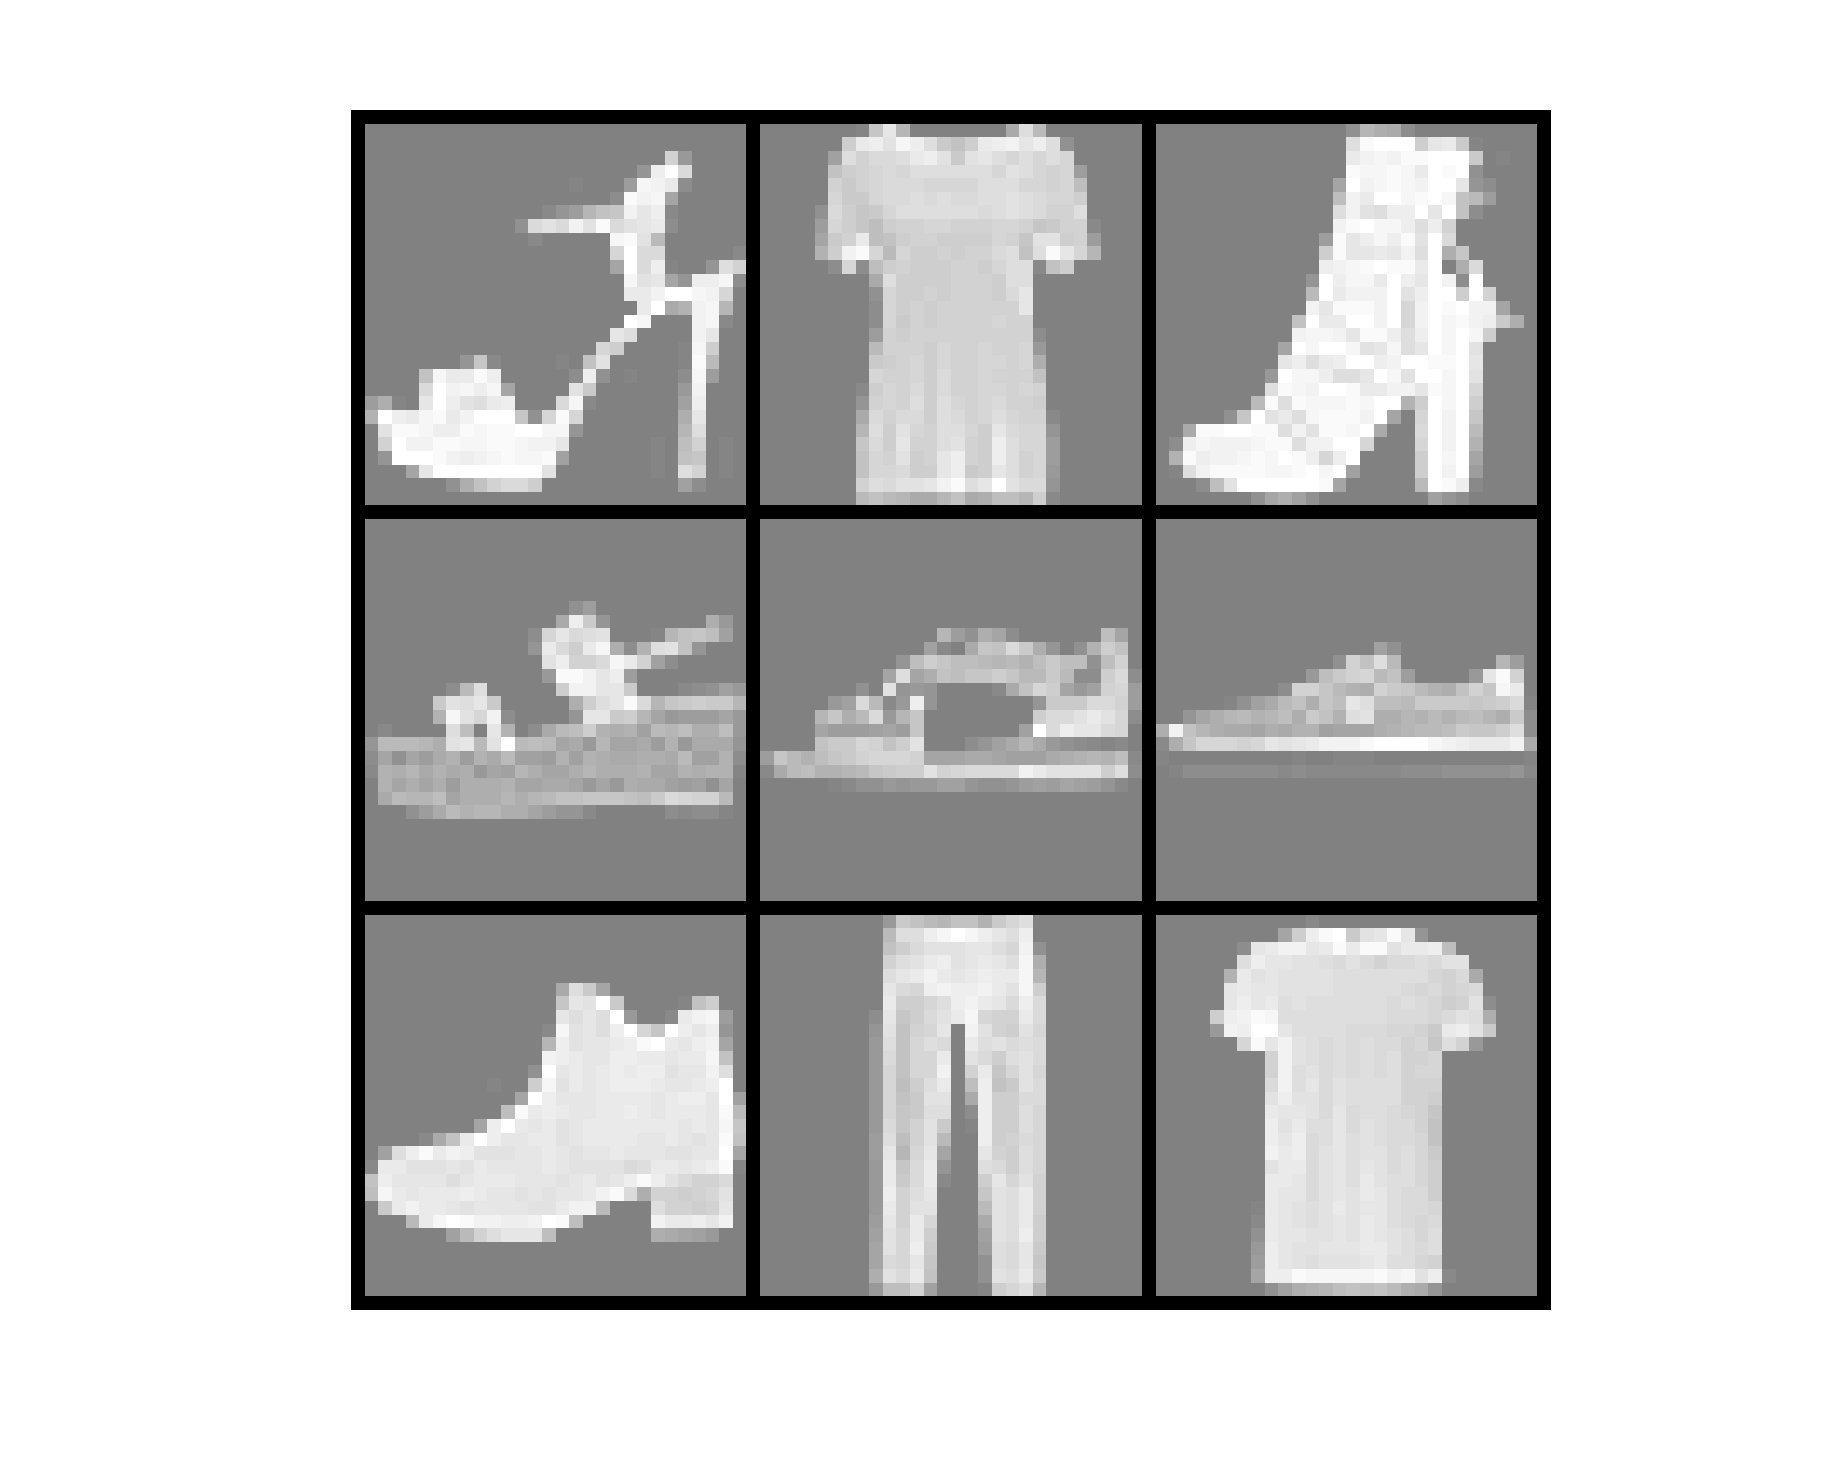
\includegraphics[width=\linewidth]{fashion_raw}
  \caption{~}
\end{subfigure}%
\begin{subfigure}{.5\textwidth}
  \centering
  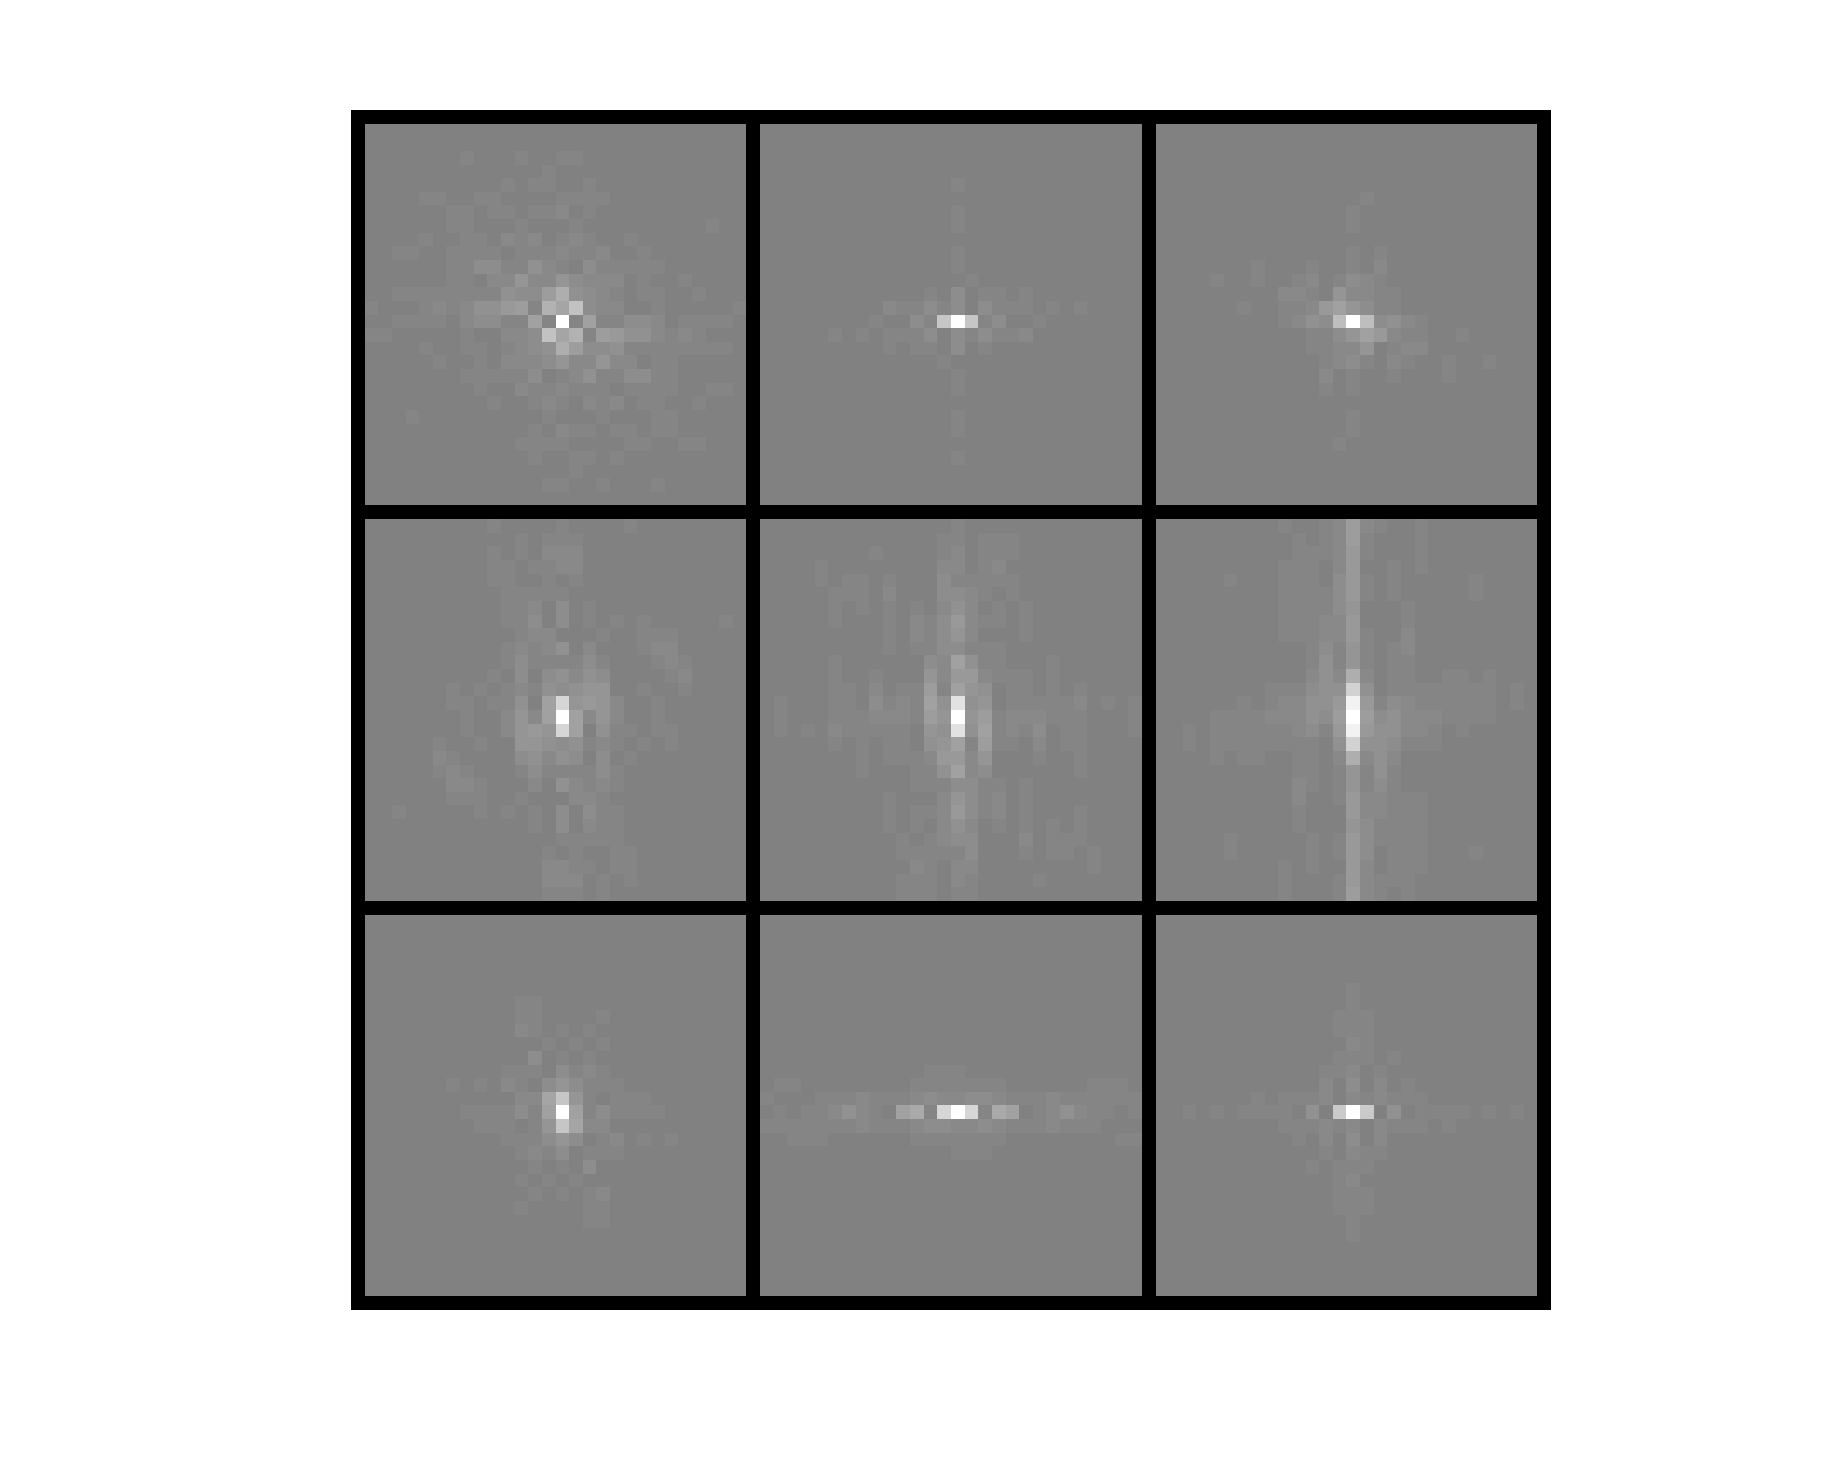
\includegraphics[width=\linewidth]{fashion_ft2}
  \caption{~}
\end{subfigure}
\vspace{1em}
\caption{Some images from the Fashion MNIST dataset (a), and their respective frequency decomposition through the 2D Fourier Transform (b).}
	\end{figure}
\end{frame}

\begin{frame}
\frametitle{Results - PCA + 1D Neural Network - Fashion MNIST}
\begin{table}[hbt]
  \begin{tabular}{|cc|l|c|c|}
  	\hline
    \% Var & PCs & NN Architecture & Training Error & Test Error \\
    \hline
    \hline
    50 &2 & 25-15 & 0.498     & 0.516\\
    50 & 2 & 10 & 0.52256     & 0.554\\
    \hline
    75 & 3 & 100 & 0.35622    &  0.398\\
    75 & 3 & 25 & 0.40367   &   0.422\\
    \hline
    85 & 8 & 100-50-20 & 0.22089    &  0.257\\
    85 & 8 & 10 & 0.28756    &  0.327\\
    \hline
    95 & 44 & 25-15 & 0.17978    &  0.399 \\
    95 & 44 & 100 & 0.151   &   0.444\\
    \hline
  \end{tabular}
    \vspace{1em}
  \caption{Best and worst results for different PCA sizes depending on explanatory power of the variance. The dataset is preprocessed by doing 2D Fourier transform of each image. Training size: 9000 images. Test size: 1000 images.}
\end{table}
\end{frame}

\subsection{CNN}

\begin{frame}[standout]
	\centering
	\textit{Results}\\
	\vspace{2em}
	\textbf{CNN}
\end{frame}

\begin{frame}
\frametitle{Results - CNN - MNIST}
\begin{table}[hbt]
  \begin{tabular}{|c|l|c|c|}
  	\hline
    \# & CNN Architecture & Training Error & Test Error\\
    \hline
    \hline
        1 & 2D(5x5,4)  &                 0.025625   &  0.055\\     
    2 & 2D(5x5,8)  &               0.020375  &   0.049  \\   
    3 & 2D(3x3,4)-BN      &          0.002125  &   0.045   \\  
    4 & 2D(3x3,8)-BN-2D(5x5,16)-BN      &        0.001625  &   0.031 \\
    \hline
  \end{tabular}
  \vspace{2em}
  \caption{{Training size: 9000 images (10\% for validation). Training options: Stochastic Gradient Descent with Momentum, maximum 20 epochs with validation patience of 10 epochs, Mini Batch size of 64, L2 regularization factor of 0.0005.}}
\end{table}
\end{frame}

\begin{frame}
\frametitle{Results - CNN - notMNIST}
\begin{table}[hbt]
  \begin{tabular}{|c|l|c|c|}
  	\hline
    \# & CNN Architecture & Training Error & Test Error\\
    \hline
    \hline
       1 & 2D(5x5,4)     &              0.08275   &  0.112  \\   
   2 & 2D(5x5,8)   &         0.08125     &0.108  \\   
    3 & 2D(3x3,4)-BN     &       0.044875    & 0.099 \\    
    4 & 2D(3x3,8)-BN-2D(5x5,16)-BN     &        0.0415    & 0.088   \\
    \hline
  \end{tabular}
  \vspace{2em}
  \caption{{Training size: 9000 images (10\% for validation). Training options: Stochastic Gradient Descent with Momentum, maximum 20 epochs with validation patience of 10 epochs, Mini Batch size of 64, L2 regularization factor of 0.0005.}}
\end{table}
\end{frame}

\begin{frame}
\frametitle{Results - CNN - Fashion MNIST}
\begin{table}[hbt]
  \begin{tabular}{|c|l|c|c|}
  	\hline
    \# & CNN Architecture & Training Error & Test Error\\
    \hline
    \hline
    1 & 2D(5x5,4)   &             0.16287    &  0.179     \\
    2 & 2D(5x5,8)   &            0.16225     & 0.168     \\
   3 & 2D(3x3,4)-BN   &           0.1035      &0.148   \\  
    4 & 2D(3x3,8)-BN-2D(5x5,16)-BN    &           0.10475      &0.144  \\
    \hline
  \end{tabular}
  \vspace{2em}
  \caption{{Training size: 9000 images (10\% for validation). Training options: Stochastic Gradient Descent with Momentum, maximum 20 epochs with validation patience of 10 epochs, Mini Batch size of 64, L2 regularization factor of 0.0005.}}
\end{table}
\end{frame}

\begin{frame}[standout]
	\centering
	\textbf{Thank You}
\end{frame}

\end{document}